\documentclass[../report.tex]{subfiles}
\begin{document}
    \begin{frame}
    	\frametitle{2a)Template Matching - TL}
    	\begin{table}[!htb]
        \centering
        \begin{tabular}{ c m{5cm} }
        
            \begin{minipage}{.45\textwidth}
            \frame{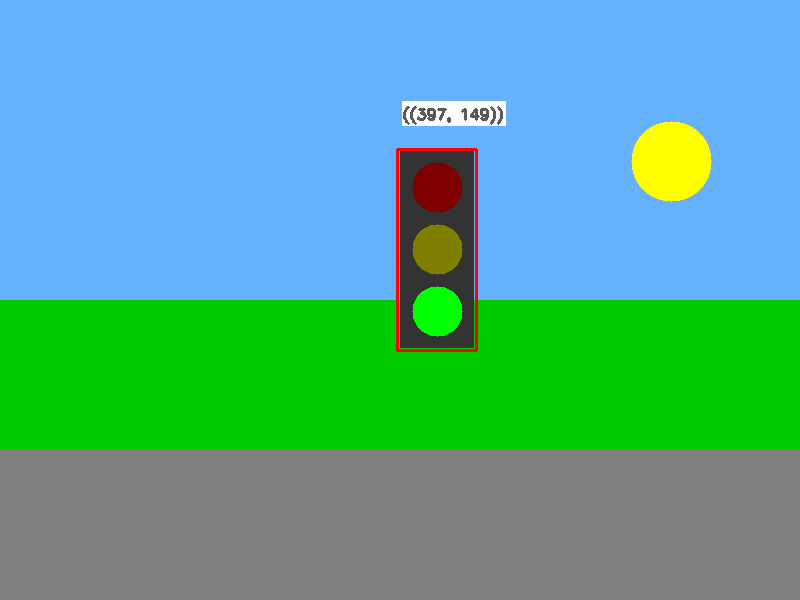
\includegraphics[keepaspectratio,height=0.7\textheight,width=1\textwidth]{output/ps2-2-a-1.jpg}}
                \captionof{figure}{ps2-2-a-1}
            \end{minipage}
            &
            \begin{minipage}{.45\textwidth}
                \selectfont\textcolor{blue}{Coordinates:} \\
                (-1, -1)
            \end{minipage}
        
        \end{tabular}
        \end{table}
    \end{frame}
    
    \begin{frame}
    	\frametitle{2b)Template Matching - Construction}
    	\begin{table}[!htb]
        \centering
        \begin{tabular}{ c m{5cm} }
        
            \begin{minipage}{.45\textwidth}
            \frame{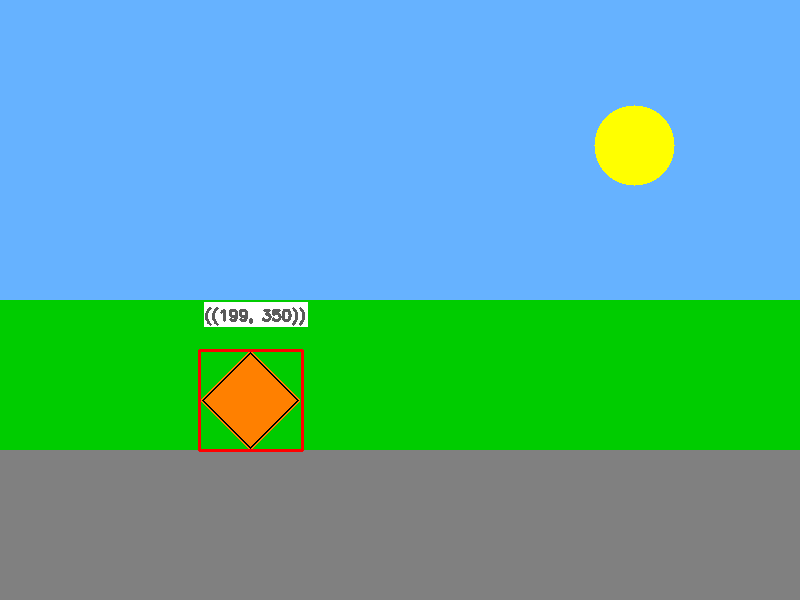
\includegraphics[keepaspectratio,height=0.7\textheight,width=1\textwidth]{output/ps2-2-b-1.jpg}}
                \captionof{figure}{ps2-2-b-1}
            \end{minipage}
            &
            \begin{minipage}{.45\textwidth}
                \selectfont\textcolor{blue}{Coordinates:} \\
                (-1, -1)
            \end{minipage}
        
        \end{tabular}
        \end{table}
    \end{frame}
    
    \begin{frame}
    	\frametitle{2c)Template Matching - Finding Waldo}
    	\begin{table}[!htb]
        \centering
        \begin{tabular}{ c m{5cm} }
        
            \begin{minipage}{.45\textwidth}
            \frame{\includegraphics[keepaspectratio,height=0.7\textheight,width=1\textwidth]{output/ps2-2-c-1.jpg}}
                \captionof{figure}{ps2-2-c-1}
            \end{minipage}
            &
            \begin{minipage}{.45\textwidth}
                \selectfont\textcolor{blue}{Coordinates:} \\
                (-1, -1)
            \end{minipage}
        
        \end{tabular}
        \end{table}
    \end{frame}
    
    \begin{frame}[t]
		\frametitle{2d)Discussion}
		
		\begin{normalsize}
			\begin{itemize}
				\setlength\itemsep{1em}\fontsize{6pt}{6pt}
				
				\item[] \textbf{
					What are the disadvantages of using Hough based methods in finding Waldo? Can template matching be generalised to all images? Explain Why/Why not. Which method consistently performed the best, why?
				 }

				\item[] {\selectfont\textcolor{blue}{Answer here.}}

			\end{itemize}
		\end{normalsize}
		
	\end{frame}
    
\end{document}